\begin{figure}
  \oneCol{0.46}
  {
    \underline{$\Rep^R(\col)$}\\[2pt]
    $\salt \getsr \bits^\lambda$;
    $M \gets \sum_{x \in \col} \cmap_m(R(x))$;
    if $w(M) > t$ then return $\bot$\\
    return $\langle M, \salt \rangle$
    \\[6pt]
    \underline{$\Qry^R(\langle M, \salt \rangle,x)$}\\[2pt]
    return $[w(B_m(R(x)) \wedge M) = k]$
    \\[6pt]
    \underline{$\Up^R(\langle M, \salt \rangle,x)$}\\[2pt]
    if $\hw(M) > t$ then return $\bot$\\
    return $M + \cmap_m(R(x))$
  }
  \caption{The formal definition of $\BF[R,t,\lambda] = (\Rep^R,\Qry^R,\Up^R)$
  for function $R: \bits^* \to [m]^k$ and natural numbers $t, \lambda$. Here,
  $\hw$ is a function counting the number of nonzero counters and $\cmap_m$ is a function taking a list $L$
  of indices in $[m]$ and producing an array $A$ of length $m$ such that $A[i]$ counts the number of times $i$ appears in $L$.}
  \label{fig:bcf-def}
\end{figure}

A modification of the Bloom filter construction known as the counting filter is given in~\ref{fig:cbf-def}. Once again we can consider different variants depending on whether or not a salt and/or key is present. From this
general construction we specify three specific structures to focus on. The first
is the `bad' unsalted and unkeyed Bloom filter $\BF[H,t]$ for some hash
function $H: \bits^* \to [m]^k$, which is defined as $\BF[H,t,0]$. The `salted'
Bloom filter is the same except for allowing a nontrivial salt, so that
$\SBF[H,t,\lambda]$ for a hash function $H$ is just $\BF[H,t,\lambda]$. Finally,
the `keyed' bloom filter $\SKBF[F_K,t,\lambda]$ is $\BF[F_K,t,\lambda]$, where
$F: \keys \times \bits^* \to [m]^k$ is a pseudorandom function with thev same key space as the data structure.

Because a counting filter without deletion behaves identically (in terms of
responding to queries) to a standard Bloom filter, any attack on a Bloom filter
works equally well against a counting filter. This means that the adversarial
advantage against a counting filter, under any of the correctness notions and
using any parameters, is bounded below by the advantage against a Bloom filter
with the same parameters.

This lower bound is not tight, however, since there are some attacks which
exploit the more powerful $\UPO$ oracle provided to the adversary in the case of
a counting filter. For example, while a salted and keyed Bloom filter is secure even in the public representation case, a salted and keyed counting filter is not secure in the same setting. The attack against a keyed but unsalted Bloom filter can be modified to work in this setting. That attack involved calling $\REPO$ several times to determine representations of singletons from some set $\setT$, from which the adversary could determine for itself what the representation of any subset of $\setT$ would look like. While the presence of a salt prevents this attack from working, in the case of a counting Bloom filter we can modify the attack to work even if a salt is used. Specifically, instead of calling $\REPO$ several times to determine the singleton representations, the adversary calls $\REPO$ only once to get an empty representation, and then uses pairs of $\UPO$ calls to insert and then delete the elements of $\setT$. In this way, the adversary will be able to see the representation of each singleton subset of $\setT$, and then perform offline computations to find subsets $\setR, \setS \subset \setT$ such that the elements of $\setR$ produce errors when queried for in the representation of $\setS$. Once the adversary has determined this, it can use $\UPO$ to insert the elements of $\setS$ and query the elements of $\setR$ in order to win the game. The use of a salt is irrelevant to this attack since only a single representation is ever used, and only $2|\setT|+|\setS|$ calls to $\UPO$ and $|\setR|$ calls to $\QRYO$ are used.

Because of this, using a private representation is necessary to obtain good bounds for a counting filter. In order to prevent possible pollution attacks, where the adversary inserts elements in such a way as to minimize the number of nonzero counters, we also use a thresholding assumption. This introduces an additional parameter $p \in [0,1]$, such that we reject any update that would cause the proportion of nonzero counters in the filter to exceed $p$. Using these two assumptions, we can derive a
false positive bound similar to that of a salted standard Bloom filter.

Unlike with a standard Bloom filter, the choice of error function is nontrivial. While we are assuming that $d(x,x)$ is always 0, so that the adversary does not get credit for a correct query, it is possible that $d(0,1)$ (the weight of a false negative) may be different than $d(1,0)$ (the weight of a false positive).

\begin{theorem}[Correctness Bound for Counting Filters]\label{thm:count-bf-bound}
Fix integers $k, m, n, \lambda, r\geq 0$ and an error function $d$, and let $\Pi$ be a .
  For every $t, q_R, q_T, q_U, q_H \geq 0$, it holds that
  \begin{eqnarray*}
    \Adv{\erreps}_{\struct,r}(t,&q_R,& q_T, q_U, q_H) \leq \\ && q_R \cdot \left[\frac{q_H}{2^\lambda} + \binom{q_T}{\mu}\left(p+\frac{k\mu}{m}\right)^{k\mu}\right] \,,
\end{eqnarray*}
where $\mu = \lceil r/\max(k \cdot d(0,1), d(1,0)) \rceil$
\end{theorem}

\begin{figure*}
  \boxThmBFSaltCorrect{0.48}
  {
    \underline{$\game_0(\advA)$}\\[2pt]
      $\col \getsr \advA^H$; $\setC \gets \emptyset$; $\setB \gets \col$; $\err \gets 0$\\
      $\pub \getsr \Rep[\HASHO](\col)$\\
      $\bot \getsr \advA^{\HASHO,\QRYO,\UPO,\INTO}$\\
      return $(\err \geq r)$
    \\[6pt]
    \oraclev{$\QRYO(x)$}\\[2pt]
      $\setB \gets \setB \cup x$\\
      if $x \in \mathcal{C}$ then return $\bot$\\
      $\setC \gets \setC \union \{x\}$\\
      $a \gets \Qry[\HASHO](\pub, x)$\\
      if $a \neq [x \in \col]$ then $\err \gets \err + 1$\\
      return~$a$
    \\[6pt]
    \oraclev{$\UPO(x,b)$}\\[2pt]
      $\setB \gets \setB \cup x$\\
      $\setC \gets \emptyset$\\
      $a \gets \Qry[\HASHO](\pub, \qry_x)$\\
      if $x \in \setC$ and $b = a \neq [x \in \col]$ then\\
      \tab $\err \gets \err-1$\\
      if $b = 1$ then\\
      \tab $\col \gets \col + \{x\}$\\
      else\\
      \tab $\col \gets \col - \{x\}$\\
      $\pub \gets \Up[\HASHO](\pub,\up_{x,b})$\\
      return~$\bot$
    \\[6pt]
    \oraclev{$\HASHO(x)$}\\
      $\hh \getsr [m]^2$; $\vv \gets \fff(\hh$)\\
      if $T[x]$ is defined then $\vv \gets T[x]$\\
      $T[x] \gets \vv$;
      return $\vv$
  }
  {
    \underline{$\game_1(\advA)$}\\[2pt]
    \oraclev{$\INTO(x,y)$}\\
      if $x \not\in \col$ or $y \not\in \col$ then\\
      \tab return $\bot$\\
      $i \gets 0$\\
      for $h$ in $\HASHO(x)$ do\\
      \tab if $h$ in $\HASHO(y)$ then $i \gets i+1$\\
      return $i$
    \\[6pt]
    \underline{$\game_2(\advA)$}\\[2pt]
    \oraclev{$\UPO(x)$}\\
      if $\QRYO(x)$ and $x \not\in \col$ then\\
      \tab $\err \gets \err + \max(k \cdot d(0,1), d(1,0))$\\
      $\setB \gets \setB \cup x$\\
      $\setC \gets \emptyset$\\
      $a \gets \Qry[H](\pub, \qry_x)$\\
      if $x \in \setC$ and $a \neq [x \in \col]$ then\\
      \tab $\err \gets \err-1$\\
      $\col \gets \col + \{x\}$\\
      $\pub \gets \Up[H](\pub,\up_{x,b})$\\
      return~$\bot$
  }
  {
  }
  {
  }
  \caption{Games 0--3 for proof of Theorem~\ref{thm:count-bf-bound}.}
  \label{fig:count-bf-bound}
\end{figure*}

\begin{proof}
Applying lemma~\ref{lemma:errep} and lemma~\ref{lemma:salttorand}, we reduce the
$\erreps$ experiment to the $\erreps1$ experiment with a salted hash function
replaced by true random sampling from $[m]$ for each of the $k$ distinct hash
values. This is given in $\game_0$. In $\game_1$, we account for the possibility
that the adversary can glean information about the overlap between sets by
querying each of them separately. In particular, we give the adversary an
additional oracle $\INTO$ that returns the number of locations in which two
elements overlap. However, we constrain $\INTO$ to only return an answer when
the element has previously been sent to some other oracle.

Because new $\QRYO$ and $\UPO$ calls are based on random sampling, this does not
provide the adversary with any additional information about how additional
elements which might be queried, inserted, or deleted in the future might
behave. However, any element which is sent to $\QRYO$ or $\UPO$ which acts as a
false positive will be immediately recognized as such. Because of this, our next
step will be to move to a game $\game_2$ where any insertion of a false positive
immediately gives the adversary credit for the worst possible error that could
be caused by either inserting or deleting that element.

Define $\delta = \max(k \cdot d(0,1), d(1,0))$ and $\mu = \lceil r/\delta
\rceil$. In $\game_2$, we modify the game so that producing a false positive
increments $\err$ by $\delta$, but so that elements cannot be removed from the
set. Because false negatives can only be produced by deleting false positives,
and the deletion of $n$ false positives can only produce as many as $nk$ false
negatives, this means that the adversary has no need to cause false negatives.
Doing so can only decrease the chances of producing additional errors by
reducing the values of counters in the filter, and so this does not decrease the
adversary's ability to produce errors. Furthermore, we increase the allowed
number of nonzero counters from $mp$ to $mp + k\lceil r/\delta \rceil$. The only
way in which not being able to remove false positives can decrease the
adversary's effectiveness is if the maximum capacity of the filter is reached.
Since each false positive removed causes $k$ nonzero counters to be returned to
zero, and the adversary stops after accumulating $r$ errors, an allowance of an
extra $k\lceil r/\delta \rceil$ nonzero counters is enough to make up for this.

Since each new element queried from outside $\col$ has its corresponding indices
determined by a true random function, the adversary can do no better than
maximizing the number of nonzero counters in its attempt to produce false
positives. Assuming the adversary is able to achieve a maximum-capacity number
of nonzero counters, the probability of any particular counter being nonzero is
$(mp + k\lceil r/\delta \rceil)/m = p +
\frac{k}{m}\lceil\frac{r}{\delta}\rceil$. Over $k$ total hashes, the probability
of a false positive is $\left((mp + k\lceil r/\delta \rceil)/m = p +
\frac{k}{m}\lceil\frac{r}{\delta}\rceil\right)^k$. Since the adversary needs to
accumulate $\lceil\frac{r}{\delta}\rceil$ errors over the course of $q_T$
queries, the probability of the adversary succeeding in this game is

$$\Prob{\game_2(\advA) = 1} = \binom{q_U + q_T}{\mu}\left(p+\frac{k\mu}{m}\right)^{k\mu}$$

Therefore the advantage of the adversary in the original game is

$$\Adv{\erreps}_{\struct_s,r}(\advA) \le q_R \cdot \left(\frac{q_H}{2^\lambda} + \binom{q_T}{\mu}\left(p+\frac{k\mu}{m}\right)^{k\mu}\right).$$

%\missingqed

\end{proof}

For concrete error bounds, we assume that $d(0,1) = d(1,0) = 1$, so that $\mu =
\lceil r/k \rceil$. The default parameters are the same as in the case of an
ordinary Bloom filter.

%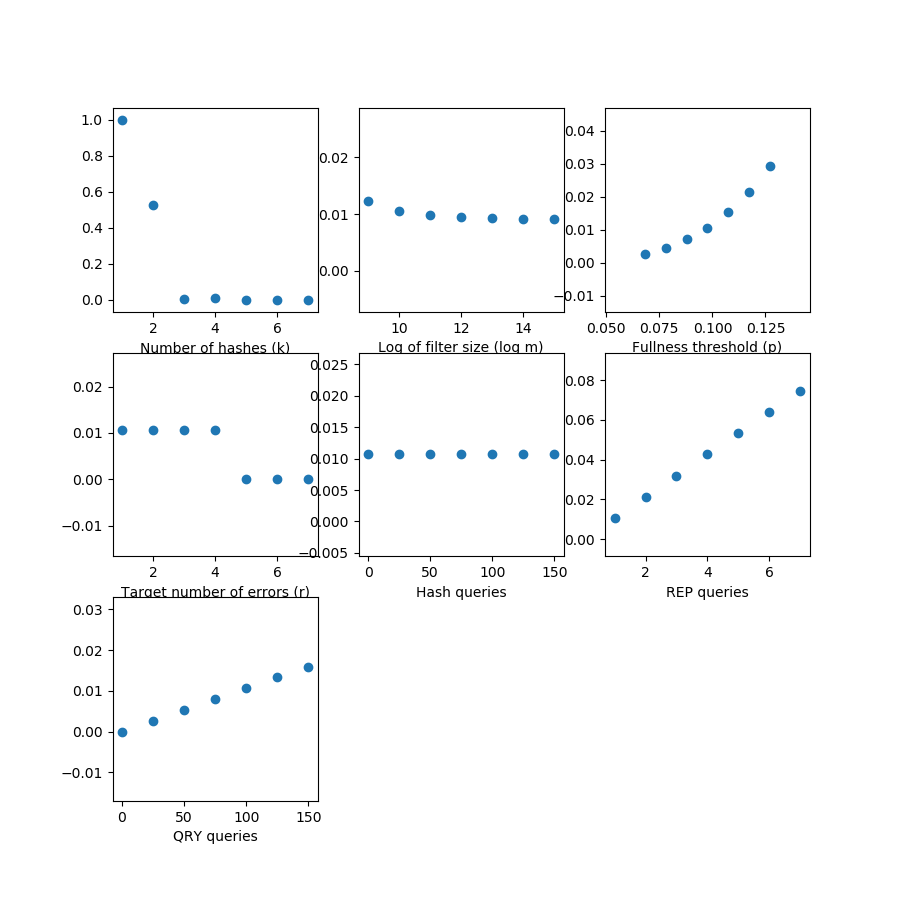
\includegraphics[scale=0.75]{CBF_Fig}

%\subsection{Attack on Counting Filters}

%First, $\advA$ chooses an arbitrary set $\col$ of size $n$ and calls $\REPO$ to get a representation of $\col$. The adversary then chooses $q_U$ distinct elements not in $\col$ and makes a series of $\UPO$ calls to remove each of these from the set. Finally, the adversary chooses up to $q_T$ elements from $\col$ and makes a series of $\QRYO$ calls to test for membership of these elements in the set.

%\begin{tabular}{|l|} 
% \hline
% \underline{adversary $\advA$:}\\
% $\col \gets [n]$\\
% $\REPO(\col)$\\
% for $i \in [q_U]$ do\\
% \tab $\UPO(0,\up_{i+n}')$\\
% for $j \in [q_T]$ do\\
% \tab $\QRYO(0,\qry_{j})$\\
% return 0\\
% \hline
%\end{tabular}